%% =============================================================
%%  Les cadences
%%  Guide de référence, composé en LaTeX, gravures LilyPond
%% =============================================================
%%
%%  Les figures (gravures/ca-*.cropped.pdf), les réponses des
%%  exercices (gravures/cadences-reponses.tex) et le fichier
%%  cadences.musicxml sont produits par outils/generer_cadences.py, à
%%  partir du modèle de hauteurs des autres guides (outils/gammes.py,
%%  outils/intervalles.py) et de l'analyse des accords
%%  (outils/generer_accords.py). Voir le colophon en dernière page.
%%
\documentclass[a4paper,11pt]{article}

\usepackage[top=2.2cm,bottom=2.4cm,left=2.2cm,right=2.2cm]{geometry}
\usepackage[T1]{fontenc}
\usepackage[utf8]{inputenc}
\usepackage[french]{babel}
\usepackage{lmodern}
\usepackage{amsmath}
\usepackage{xcolor}
\usepackage{graphicx}
\usepackage{titlesec}
\usepackage{fancyhdr}
\usepackage{mdframed}
\usepackage{enumitem}
\usepackage{booktabs}
\usepackage{hyperref}

\graphicspath{{gravures/}}

% ---- Couleurs, reprises du document des accords de guitare ---------
\definecolor{navy}{RGB}{18,50,105}
\definecolor{lightnavy}{RGB}{235,241,255}
\definecolor{mygray}{RGB}{110,110,110}

\hypersetup{colorlinks=true, linkcolor=navy, urlcolor=navy,
  pdftitle={Les cadences},
  pdfauthor={Fabian Bastin}}

% ---- En-tête et pied -----------------------------------------------
\pagestyle{fancy}
\fancyhf{}
\renewcommand{\headrulewidth}{0.4pt}
\renewcommand{\footrulewidth}{0.4pt}
\fancyhead[L]{\small\bfseries\textcolor{navy}{Les cadences}}
\fancyhead[R]{\small\textcolor{mygray}{\thepage}}
\fancyfoot[C]{\small\textcolor{mygray}{Les cadences}}

% ---- Titres de section ---------------------------------------------
\newcommand{\navysect}[1]{%
  \colorbox{navy}{%
    \parbox[c][17pt]{\dimexpr\linewidth-2\fboxsep\relax}{%
      \color{white}\hspace{6pt}\bfseries\normalsize #1}}%
}
\titleformat{\section}[block]{\normalfont}{}{0pt}{\navysect}
\titlespacing*{\section}{0pt}{16pt}{10pt}

% ---- Encadré de remarque -------------------------------------------
\newmdenv[linecolor=navy, linewidth=0.5pt, backgroundcolor=lightnavy,
  innertopmargin=6pt, innerbottommargin=6pt,
  innerleftmargin=8pt, innerrightmargin=8pt,
  skipabove=8pt, skipbelow=8pt, nobreak=true]{remarque}

% ---- Chiffrages ------------------------------------------------------
% Un chiffre romain et ses chiffres empilés : \ch{I}{6}{4} donne I 6 sur 4.
\newcommand{\ch}[3]{\ensuremath{\mathrm{#1}^{#2}_{#3}}}

% ---- Figure gravée ---------------------------------------------------
% Figure gravée, avec sa légende. Toutes les gravures sont à la même
% échelle, celle des gravures des accords : leurs portées ont la même
% taille, quelle que soit leur largeur. Le tout tient dans une minipage :
% figure et légende ne sont jamais séparées par un saut de page.
\newcommand{\echelle}{1.16}
\newcommand{\gravure}[2]{%
  \par\medskip\noindent
  \begin{minipage}{\linewidth}
    \centering
    \includegraphics[scale=\echelle]{#1.cropped.pdf}\\[4pt]
    {\small\itshape\color{mygray} #2}
  \end{minipage}\par\medskip
}

\setlist{itemsep=2pt, topsep=4pt, parsep=0pt}

\begin{document}

% =====================================================================
\begin{titlepage}
\centering
\vspace*{3cm}
{\Huge\bfseries\color{navy} Les cadences\par}
\vspace{1.4cm}
{\large Le V suspend, le I conclut\par}
\vspace{2.5cm}
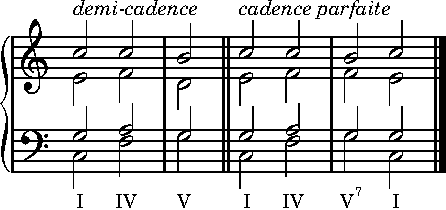
\includegraphics[scale=1.4]{ca-phrase.cropped.pdf}
\vfill
{\small\color{mygray}
Gravures LilyPond, composition \LaTeX.\\
Fichier MusicXML joint.\par}
\vspace{1cm}
\end{titlepage}

\tableofcontents
\newpage

% =====================================================================
\section{Avant-propos}

Une \textbf{cadence} est la fin d'une phrase musicale : les deux ou trois
accords sur lesquels elle se pose ou reste en suspens, comme une phrase écrite
s'achève sur un point ou s'interrompt sur une virgule. Au programme de matières
théoriques de l'École de musique Vincent-d'Indy, ces notions relèvent des
niveaux 7 et 8.

Les noms des cadences, leurs définitions et la manière de les jouer changent
d'un ouvrage à l'autre. Les pages qui suivent donnent le tronc commun, puis
les variantes, réunies à la section~\ref{sec:ouvrages} ; aucune définition n'y
est tenue pour la seule bonne.

À lire après
\href{https://www.slashbin.net/musique/theorie/accords.pdf}{\emph{Les
accords}}, qui bâtissent les accords sur chaque degré et en donnent les
chiffres, et
\href{https://www.slashbin.net/musique/theorie/tonalites.pdf}{\emph{Les
tonalités}}, où la cadence confirme une tonalité nouvelle.

\begin{remarque}
\textbf{Conventions.} Les notes sont nommées en français, et les octaves
comptées à la française : do3 est le do central. Les exemples sont écrits pour
le clavier, sur une grande portée. Sauf mention contraire, ils sont à quatre
voix, deux par main --- soprano et alto en clé de sol, ténor et basse en clé
de fa ---, en blanches ; le style clavier, trois sons à la main droite et la
basse seule, est présenté à la section~\ref{sec:clavier}. Sous la basse, le
chiffre romain du degré et le chiffrage de l'accord, comme dans \emph{Les
accords} : \ch{V}{7}{} pour la septième de dominante, \ch{II}{6}{} pour
l'accord du deuxième degré au premier renversement, \ch{I}{6}{4} pour l'accord
de tonique au deuxième. Sauf mention contraire, les exemples sont en do
majeur.
\end{remarque}

Le fichier MusicXML joint fait entendre chaque exemple ; la
section~\ref{sec:musicxml} le présente.

% =====================================================================
\section{La ponctuation de la phrase}
\label{sec:ponctuation}

\textbf{Deux accords qui décident.} Dans la musique tonale, l'accord de tonique,
I, est le repos ; celui de dominante, V, une tension qui appelle le I. Une
phrase qui s'arrête sur V reste en suspens : la cadence est \emph{suspensive},
comme une virgule ou un point d'interrogation. Une phrase qui va de V à I se
pose : la cadence est \emph{conclusive}, comme un point. La comparaison est
ancienne : Danhauser, dans sa \emph{Théorie de la musique}, notait déjà que la
ponctuation musicale se reconnaît aux cadences.

\textbf{La question et la réponse.} Deux phrases se répondent souvent ainsi : la
première s'arrête sur V, la seconde reprend le même chemin et va jusqu'au I.

\gravure{ca-phrase}{Une phrase qui suspend sur V, puis la même qui conclut sur
I : une demi-cadence, puis une cadence parfaite.}

Cinq cadences se distinguent d'ordinaire par leurs deux derniers accords et
par leur état, fondamental ou renversé : trois concluent, deux suspendent ou
détournent.

% =====================================================================
\section{Les cadences qui concluent}
\label{sec:conclure}

\textbf{La cadence parfaite.} V, puis I, tous deux à l'état fondamental : la
dominante à la basse, puis la tonique. C'est la plus conclusive des cadences,
celle qui termine un morceau. Le V peut porter sa septième, \ch{V}{7}{}, qui
renforce l'appel du I (section~\ref{sec:preparer}). Certains ouvrages
demandent en plus la tonique au soprano sur l'accord final
(section~\ref{sec:ouvrages}).

\gravure{ca-parfaite}{La cadence parfaite, avec V puis avec \ch{V}{7}{} : la
sensible, si, monte à la tonique ; la septième, fa, descend sur mi.}

\textbf{La cadence imparfaite.} V, puis I, mais l'un des deux accords au moins
est renversé ; le plus souvent, c'est le I, au premier renversement :
V--\ch{I}{6}{}. La basse ne fait plus le saut de quinte qui affirme la
tonalité, et la phrase s'arrête sans se fermer tout à fait. Le nom n'a pas le
même sens partout (section~\ref{sec:ouvrages}).

\gravure{ca-imparfaite}{La cadence imparfaite, V--\ch{I}{6}{}, après I puis
après \ch{II}{6}{}.}

\textbf{La cadence plagale.} IV, puis I : la sous-dominante remplace la
dominante. La sensible n'y est pas, et la conclusion est plus douce. Elle
termine bien des cantiques sur le mot \emph{amen}, d'où son nom anglais
d'\emph{Amen cadence}. Le mot \emph{plagal} vient des modes du chant grégorien
qui portaient ce nom, et dont certains concluaient ainsi.

\gravure{ca-plagale}{La cadence plagale : IV--I, la tonique gardée en place au
soprano.}

% =====================================================================
\section{Les cadences qui suspendent}
\label{sec:suspendre}

\textbf{La demi-cadence.} La phrase s'arrête sur V, quel que soit l'accord qui
le précède : I, IV ou \ch{II}{6}{}, par exemple. On l'appelle aussi
\emph{cadence à la dominante}. Elle laisse l'oreille dans l'attente du I, qui
viendra avec la phrase suivante.

\gravure{ca-demi}{La demi-cadence, depuis I, depuis IV et depuis
\ch{II}{6}{}.}

\textbf{La cadence rompue.} V, puis un autre accord que le I attendu, le plus
souvent VI. L'oreille est trompée sans être perdue : VI partage deux notes avec
I, la tonique et la médiante, et la sensible monte toujours à la tonique. La
phrase doit aller chercher sa conclusion plus loin ; la cadence rompue relance
le discours, et parfois une modulation. On la dit aussi \emph{évitée}, avec
des nuances selon les ouvrages (section~\ref{sec:ouvrages}).

\gravure{ca-rompue}{La cadence rompue, depuis IV puis depuis la quarte et
sixte : la sensible monte, l'alto et le ténor descendent, et la tierce de VI,
do, est doublée.}

% =====================================================================
\section{En mineur}
\label{sec:mineur}

\textbf{La sensible haussée.} Les cadences du mineur se bâtissent sur la gamme
mineure harmonique. Son septième degré, haussé par une altération accidentelle,
est la sensible : il donne au V un accord parfait majeur, et à la cadence
parfaite la même force qu'en majeur. Sans elle, le V serait mineur, et la
cadence beaucoup plus faible.

\textbf{Les autres degrés.} I et IV sont mineurs, VI est majeur, et II est un
accord de quinte diminuée : on l'emploie au premier renversement,
\ch{II}{6}{}, où la quinte diminuée ne se fait plus entendre contre la basse.
Dans la cadence rompue, VI est à un demi-ton au-dessus de la dominante : la
basse monte d'un demi-ton.

\gravure{ca-mineur}{En la mineur, la cadence parfaite, puis la cadence rompue :
sol dièse, la sensible, monte à la tonique.}

\textbf{La seconde augmentée.} Entre le sixième degré et la sensible, la gamme
harmonique place une seconde augmentée --- fa et sol dièse en la mineur. Aucune
voix ne la parcourt : la sensible monte à la tonique, et le sixième degré
descend.

\textbf{La tierce picarde.} Un morceau mineur peut finir sur un accord de
tonique majeur : c'est la tierce picarde, que présentent
\href{https://www.slashbin.net/musique/theorie/tonalites.pdf}{\emph{Les
tonalités}}.

% =====================================================================
\section{Préparer la cadence}
\label{sec:preparer}

\textbf{Une sous-dominante avant le V.} La cadence ne se réduit pas à ses deux
derniers accords : le V est le plus souvent amené par un accord de
sous-dominante, IV ou \ch{II}{6}{}. Les deux ont le quatrième degré à la basse,
qui monte d'un ton vers la dominante.

\gravure{ca-preparer}{La cadence parfaite amenée par \ch{II}{6}{} : fa, à la
basse, monte sur sol.}

\textbf{La septième de dominante.} \ch{V}{7}{} ajoute au V sa septième, le
quatrième degré, et renforce l'appel du I : la sensible monte à la tonique, la
septième descend d'un degré. Venue de IV, cette septième est déjà là : elle
reste en place, puis descend. À quatre voix, \ch{V}{7}{} perd souvent sa
quinte ; sa fondamentale est alors doublée. Complet, il se résout plutôt sur
un I sans quinte, à la fondamentale triplée.

\textbf{La quarte et sixte de cadence.} Avant le V, un accord de tonique au
deuxième renversement, \ch{I}{6}{4}, a la dominante à la basse : sol, do et mi
en do majeur. Il tombe sur le temps fort et se résout sur V : la quarte, do,
descend sur la tierce, si ; la sixte, mi, descend sur la quinte, ré. C'est en
réalité un V dont deux notes sont retardées, une double appogiature. Sa basse
est doublée ; si vient \ch{V}{7}{}, la basse doublée descend sur la septième,
fa. Dans les exemples, la basse descend en plus à l'octave au moment du V.

\gravure{ca-quarte-sixte}{La quarte et sixte de cadence, vers V puis vers
\ch{V}{7}{} : la quarte et la sixte descendent sur la tierce et la quinte ;
vers \ch{V}{7}{}, sol, doublé, descend sur fa.}

\begin{remarque}
\textbf{\ch{I}{6}{4} ou \ch{V}{6}{4}.} Le chiffrage varie avec l'analyse : on
écrit \ch{I}{6}{4} pour l'accord qu'on lit, ou \ch{V}{6}{4}--\ch{}{5}{3} pour la
fonction qu'il remplit, celle d'un V retardé. Les gravures suivent le premier
usage, celui de \emph{Les accords}.
\end{remarque}

% =====================================================================
\section{Des enchaînements courants}
\label{sec:courants}

Quelques enchaînements reviennent sans cesse, dans les morceaux comme dans les
exercices d'harmonie. En voici six parmi d'autres, chacun terminé par l'une
des cadences qui précèdent :

\begin{itemize}
  \item I--IV--\ch{V}{7}{}--I et \ch{II}{6}{}--\ch{I}{6}{4}--\ch{V}{7}{}--I :
    cadence parfaite ;
  \item I--IV--V--VI et \ch{II}{6}{}--\ch{I}{6}{4}--V--VI : cadence rompue ;
  \item I--IV--\ch{II}{6}{}--V : demi-cadence ;
  \item I--\ch{II}{6}{}--V--\ch{I}{6}{} : cadence imparfaite.
\end{itemize}

À l'oreille, deux questions aident à les distinguer : le début, I ou
\ch{II}{6}{}, que trahit la quarte et sixte au deuxième accord ; puis la fin,
qui conclut, se détourne ou reste en suspens. La plus brève des formules,
I--\ch{V}{7}{}--I, est présentée avec le style clavier
(section~\ref{sec:clavier}).

\gravure{ca-courantes-1}{En ré majeur, les trois premières formules.}

\gravure{ca-courantes-2}{Puis les trois autres.}

Les formules rompues sont gravées ici avec V ; avec \ch{V}{7}{}, la septième
descend sur la quinte de VI.

% =====================================================================
\section{Au clavier}
\label{sec:clavier}

Deux dispositions sont courantes au clavier.

\textbf{Quatre voix, deux par main.} C'est l'écriture des traités d'harmonie,
transposée au piano : la main droite tient le soprano et l'alto, la main
gauche le ténor et la basse. La basse porte la fondamentale de chaque accord,
ou le membre que demande son chiffrage. Les exemples de ces pages en suivent
aussi quelques habitudes :

\begin{itemize}
  \item \textbf{le soprano reste près de la tonique} : la tonique sur I, IV et
    VI, le deuxième degré sur II, la sensible sur V ;
  \item \textbf{les voix intérieures bougent le moins possible} : la note
    commune reste en place, les autres voix vont au plus près ;
  \item \textbf{le ténor rejoint parfois la basse} sur la même note : une
    seule tête, deux hampes, comme dans \ch{V}{7}{} venu de IV, où la quinte
    manque ;
  \item \textbf{sous la quarte et sixte}, la basse descend à l'octave pour la
    dominante.
\end{itemize}

Ces réalisations se transposent telles quelles : chaque voix garde son degré
et sa place, et seule l'armure change.

\gravure{ca-disposition}{I--IV--\ch{V}{7}{}--I en do majeur, en si bémol majeur
et en ré mineur : la même disposition, transposée.}

\textbf{Le style clavier : trois sons et une basse.} La main gauche tient la
basse seule, la fondamentale de chaque accord ; la main droite joue trois sons
serrés, dans une octave. La note du soprano dans le premier accord donne la
\emph{position} : position d'octave quand c'est la fondamentale, de tierce ou
de quinte. D'un accord au suivant, la note commune reste en place et les
autres voix vont au plus près ; quand deux accords n'ont pas de note commune,
comme IV et V, la main droite va à l'opposé de la basse. L'enchaînement revient
à sa position de départ.

\gravure{ca-clavier-positions}{I--IV--V--I en do majeur, dans les trois
positions : do reste en place de I à IV, sol de V à I ; de IV à V, la main
droite descend quand la basse monte.}

\textbf{I--\ch{V}{7}{}--I.} La plus brève des cadences parfaites se joue aussi
ainsi. La dominante, note commune, reste en place ; la tierce de I monte sur la
septième de \ch{V}{7}{}, et sa fondamentale descend sur la sensible ; puis la
septième redescend et la sensible remonte. La main droite de \ch{V}{7}{} porte
donc la fondamentale, la tierce et la septième : la quinte manque, et la
fondamentale est doublée par la basse. L'accord de tonique final est complet.

\textbf{En majeur et en mineur sur la même tonique.} La majeur et la mineur,
tonalités homonymes (\href{https://www.slashbin.net/musique/theorie/tonalites.pdf}{\emph{Les
tonalités}}), jouent le même \ch{V}{7}{} --- mi, sol dièse, si, ré, la
sensible haussée en mineur --- ; seule change la tierce de I, do dièse ou do,
avec l'armure.

\gravure{ca-clavier-v7}{I--\ch{V}{7}{}--I en position d'octave, en do majeur, en
la majeur et en la mineur. En do majeur, sol reste en place, mi monte sur fa,
la septième, et do descend sur si, la sensible ; puis fa redescend et si
remonte.}

\textbf{Dans toutes les tonalités.} Les deux tableaux qui suivent donnent
I--IV--V--I, puis I--\ch{V}{7}{}--I, en style clavier dans les trente
tonalités usuelles. Une ligne par tonique, dans l'ordre du cycle des quintes,
les dièses puis les bémols : à gauche le majeur dans ses trois positions, à
droite le mineur homonyme, sur la même tonique. En mineur, V est majeur grâce à
la sensible haussée, et IV est mineur.

\par\medskip\noindent\textbf{I--IV--V--I, à trois sons et une basse.}\par\smallskip
%% Produit par outils/generer_cadences.py — ne pas modifier à la main.
\noindent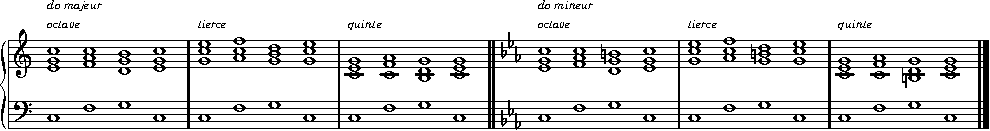
\includegraphics[width=\linewidth]{ca-tab-iv-do.cropped.pdf}\par\medskip
\noindent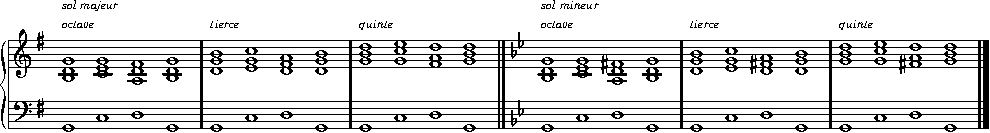
\includegraphics[width=\linewidth]{ca-tab-iv-sol.cropped.pdf}\par\medskip
\noindent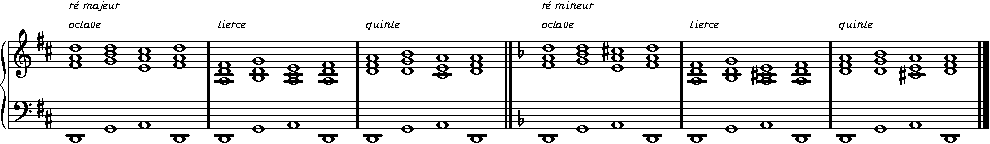
\includegraphics[width=\linewidth]{ca-tab-iv-re.cropped.pdf}\par\medskip
\noindent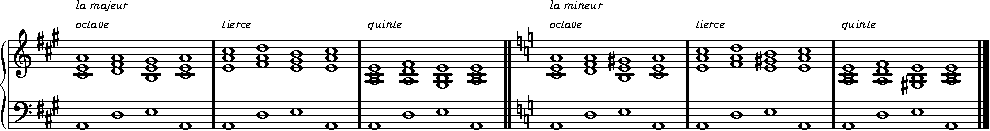
\includegraphics[width=\linewidth]{ca-tab-iv-la.cropped.pdf}\par\medskip
\noindent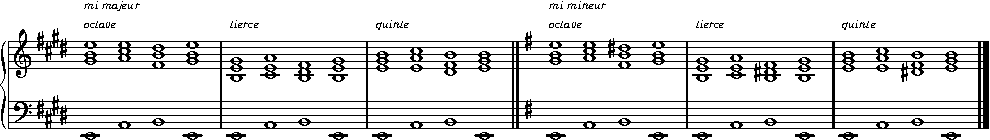
\includegraphics[width=\linewidth]{ca-tab-iv-mi.cropped.pdf}\par\medskip
\noindent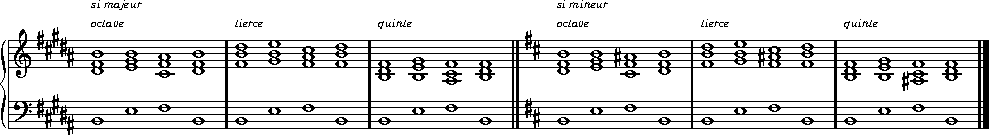
\includegraphics[width=\linewidth]{ca-tab-iv-si.cropped.pdf}\par\medskip
\noindent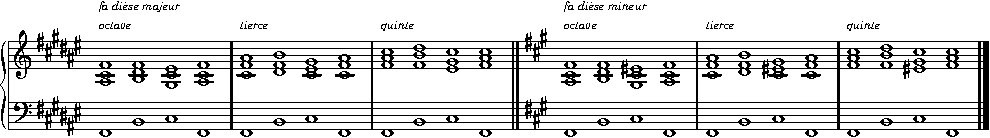
\includegraphics[width=\linewidth]{ca-tab-iv-fa-diese.cropped.pdf}\par\medskip
\noindent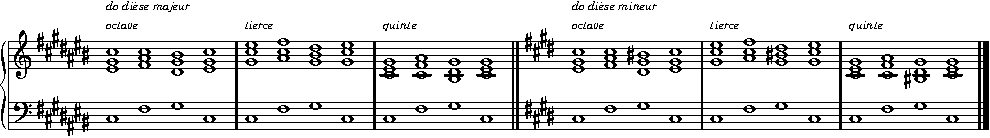
\includegraphics[width=\linewidth]{ca-tab-iv-do-diese.cropped.pdf}\par\medskip
\noindent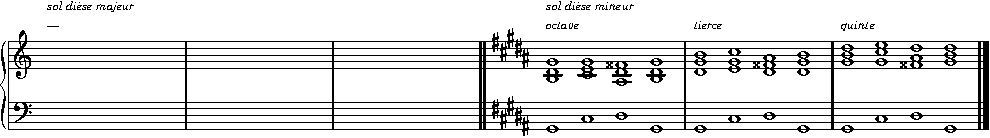
\includegraphics[width=\linewidth]{ca-tab-iv-sol-diese.cropped.pdf}\par\medskip
\noindent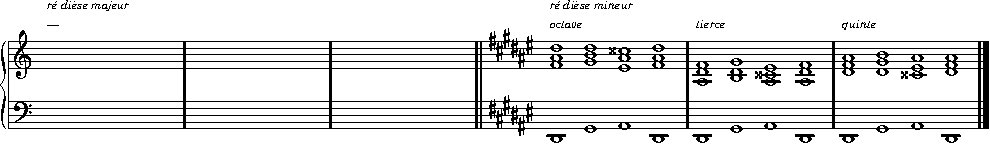
\includegraphics[width=\linewidth]{ca-tab-iv-re-diese.cropped.pdf}\par\medskip
\noindent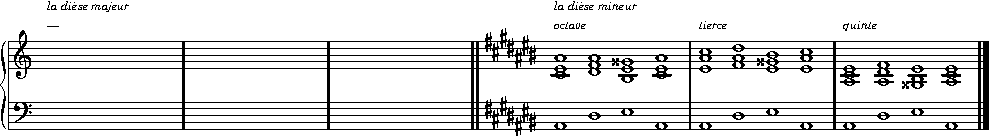
\includegraphics[width=\linewidth]{ca-tab-iv-la-diese.cropped.pdf}\par\medskip
\noindent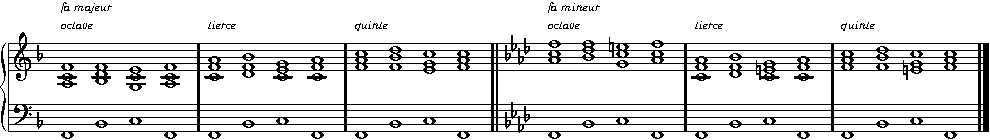
\includegraphics[width=\linewidth]{ca-tab-iv-fa.cropped.pdf}\par\medskip
\noindent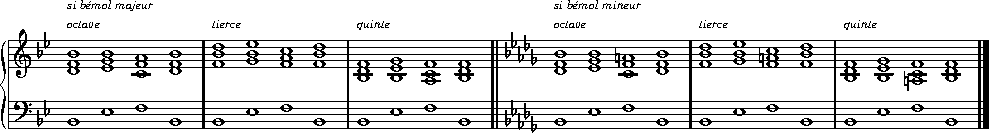
\includegraphics[width=\linewidth]{ca-tab-iv-si-bemol.cropped.pdf}\par\medskip
\noindent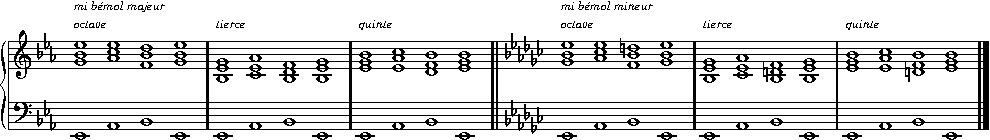
\includegraphics[width=\linewidth]{ca-tab-iv-mi-bemol.cropped.pdf}\par\medskip
\noindent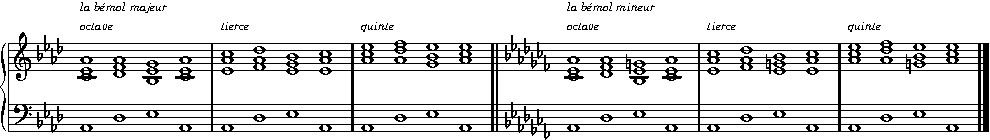
\includegraphics[width=\linewidth]{ca-tab-iv-la-bemol.cropped.pdf}\par\medskip
\noindent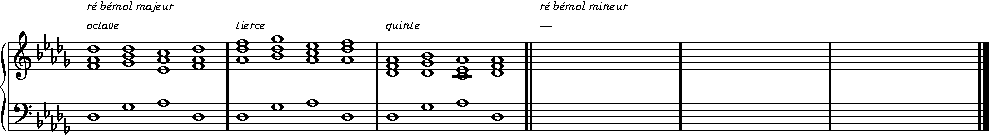
\includegraphics[width=\linewidth]{ca-tab-iv-re-bemol.cropped.pdf}\par\medskip
\noindent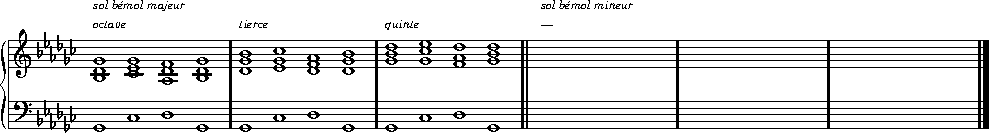
\includegraphics[width=\linewidth]{ca-tab-iv-sol-bemol.cropped.pdf}\par\medskip
\noindent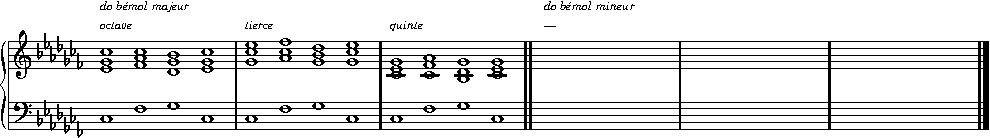
\includegraphics[width=\linewidth]{ca-tab-iv-do-bemol.cropped.pdf}\par\medskip


Les cases vides sont celles des tonalités dont l'armure compterait plus de
sept altérations : sol dièse, ré dièse et la dièse majeurs, ré bémol, sol
bémol et do bémol mineurs. On les écrit sous leur nom enharmonique : la bémol,
mi bémol et si bémol majeurs, do dièse, fa dièse et si mineurs
(\href{https://www.slashbin.net/musique/theorie/intervalles.pdf}{\emph{Les
intervalles}}, \href{https://www.slashbin.net/musique/theorie/tonalites.pdf}{\emph{Les
tonalités}}).

\par\medskip\noindent\textbf{I--\ch{V}{7}{}--I, à trois sons et une basse.}\par\smallskip
%% Produit par outils/generer_cadences.py — ne pas modifier à la main.
\noindent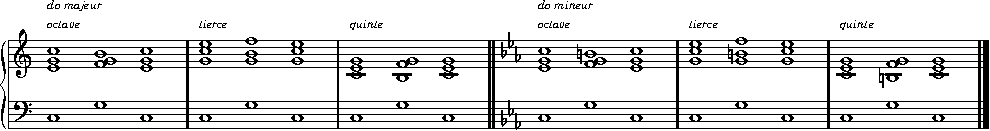
\includegraphics[width=\linewidth]{ca-tab-v7-do.cropped.pdf}\par\medskip
\noindent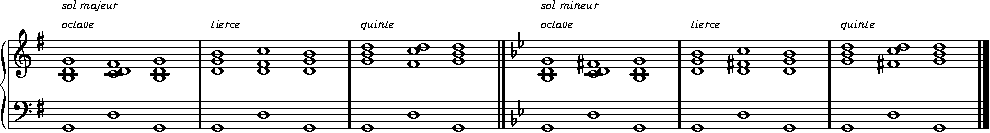
\includegraphics[width=\linewidth]{ca-tab-v7-sol.cropped.pdf}\par\medskip
\noindent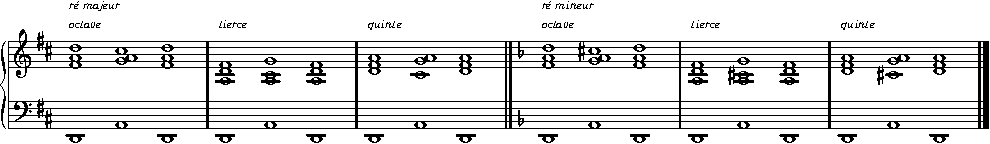
\includegraphics[width=\linewidth]{ca-tab-v7-re.cropped.pdf}\par\medskip
\noindent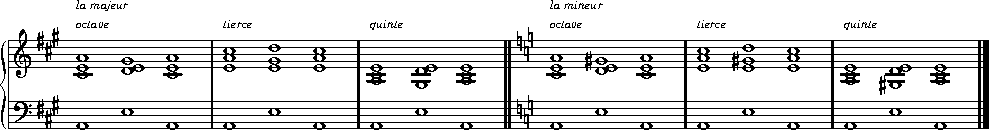
\includegraphics[width=\linewidth]{ca-tab-v7-la.cropped.pdf}\par\medskip
\noindent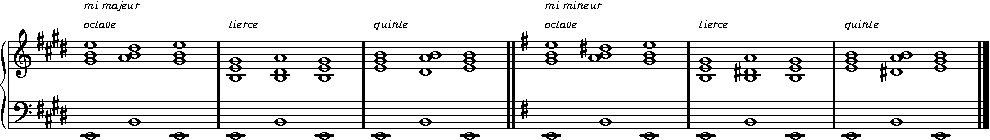
\includegraphics[width=\linewidth]{ca-tab-v7-mi.cropped.pdf}\par\medskip
\noindent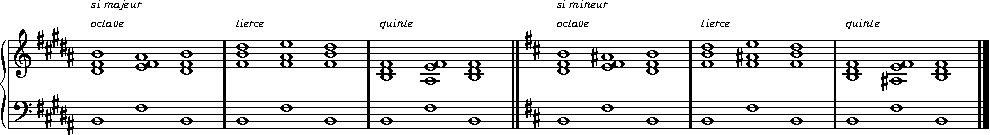
\includegraphics[width=\linewidth]{ca-tab-v7-si.cropped.pdf}\par\medskip
\noindent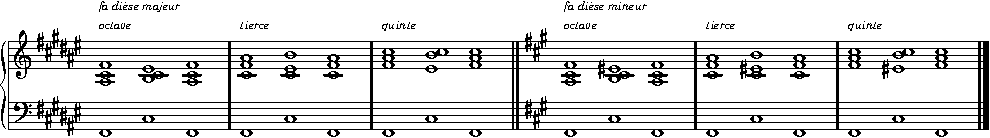
\includegraphics[width=\linewidth]{ca-tab-v7-fa-diese.cropped.pdf}\par\medskip
\noindent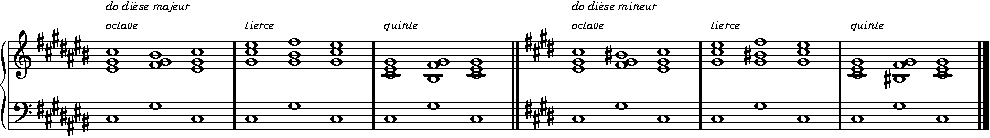
\includegraphics[width=\linewidth]{ca-tab-v7-do-diese.cropped.pdf}\par\medskip
\noindent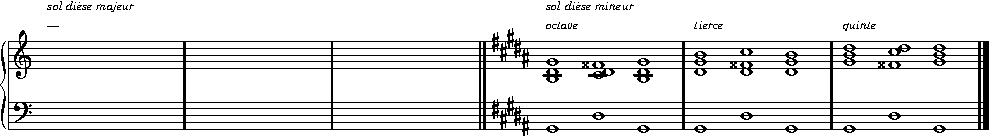
\includegraphics[width=\linewidth]{ca-tab-v7-sol-diese.cropped.pdf}\par\medskip
\noindent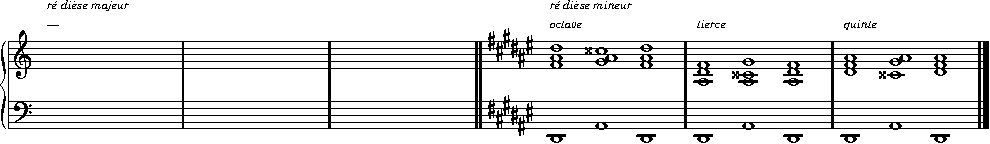
\includegraphics[width=\linewidth]{ca-tab-v7-re-diese.cropped.pdf}\par\medskip
\noindent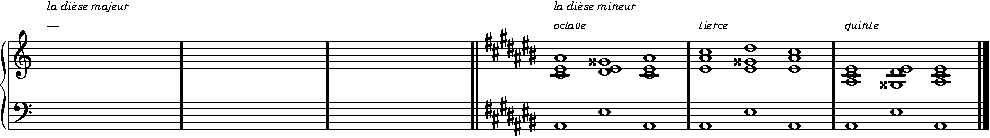
\includegraphics[width=\linewidth]{ca-tab-v7-la-diese.cropped.pdf}\par\medskip
\noindent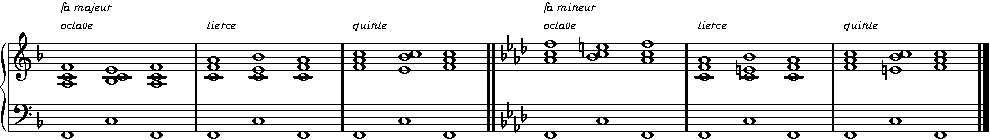
\includegraphics[width=\linewidth]{ca-tab-v7-fa.cropped.pdf}\par\medskip
\noindent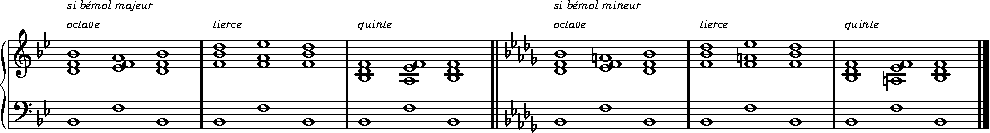
\includegraphics[width=\linewidth]{ca-tab-v7-si-bemol.cropped.pdf}\par\medskip
\noindent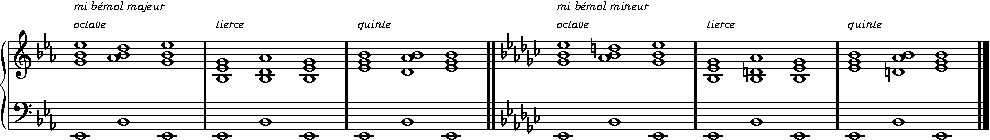
\includegraphics[width=\linewidth]{ca-tab-v7-mi-bemol.cropped.pdf}\par\medskip
\noindent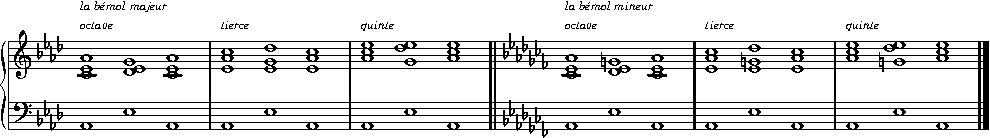
\includegraphics[width=\linewidth]{ca-tab-v7-la-bemol.cropped.pdf}\par\medskip
\noindent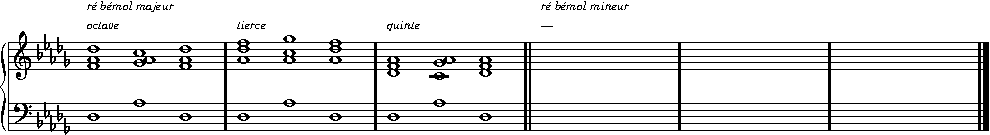
\includegraphics[width=\linewidth]{ca-tab-v7-re-bemol.cropped.pdf}\par\medskip
\noindent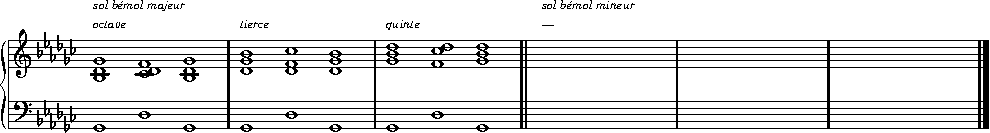
\includegraphics[width=\linewidth]{ca-tab-v7-sol-bemol.cropped.pdf}\par\medskip
\noindent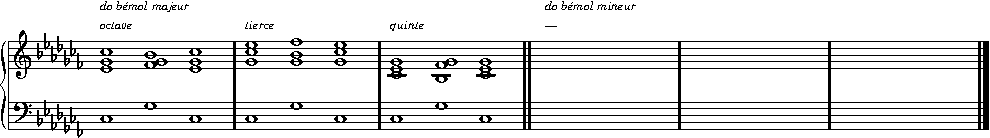
\includegraphics[width=\linewidth]{ca-tab-v7-do-bemol.cropped.pdf}\par\medskip


Les mêmes cases restent vides, pour la même raison.

% =====================================================================
\section{Les règles des voix}
\label{sec:regles}

Les quatre voix d'une cadence obéissent aux règles de l'écriture à quatre
voix.

\begin{itemize}
  \item \textbf{La sensible monte} d'un demi-ton à la tonique, de V à I comme
    de V à VI.
  \item \textbf{La septième descend} d'un degré.
  \item \textbf{Pas de quintes ni d'octaves parallèles} : deux voix à la quinte
    juste, ou à l'octave, ne passent pas ensemble à une autre quinte ou une
    autre octave. Elles sonneraient comme une seule voix doublée, et la
    phrase perdrait une de ses voix.
  \item \textbf{La fondamentale se double} dans un accord à l'état
    fondamental ; dans \ch{II}{6}{}, c'est la basse, le quatrième degré ; dans
    la quarte et sixte, la basse aussi. La sensible et la septième ne se
    doublent jamais. Au VI de la cadence rompue, la tierce est doublée.
\end{itemize}

\gravure{ca-paralleles}{IV--V en suivant la basse : les trois voix du dessus
montent avec elle, quintes et octaves parallèles. En allant à l'opposé, aucune.}

% =====================================================================
\section{D'un ouvrage à l'autre}
\label{sec:ouvrages}

Les cinq noms se retrouvent partout, mais leurs définitions ne coïncident pas,
et l'anglais en a d'autres. Le tableau compare l'article «~Cadence
harmonique~» de Wikipédia, la leçon «~Les cadences~» d'\emph{Apprendre le
solfège} et l'usage anglais, américain (\emph{US}) et britannique
(\emph{GB}).

\par\medskip\noindent
\begin{minipage}{\linewidth}
\centering\small
\renewcommand{\arraystretch}{1.25}
\begin{tabular}{@{}p{0.17\linewidth} p{0.38\linewidth} p{0.4\linewidth}@{}}
\toprule
\textbf{Cadence} & \textbf{Wikipédia, \emph{Apprendre le solfège}}
  & \textbf{Anglais} \\
\midrule
parfaite & V--I, à l'état fondamental ; sur les temps forts (Wikipédia)
  & \emph{US} \emph{perfect authentic} : en plus, la tonique au soprano ;
  \emph{GB} \emph{perfect} \\
imparfaite & V--I, un accord au moins renversé, le plus souvent
  V--\ch{I}{6}{} & \emph{US} \emph{imperfect authentic} : sans la tonique au
  soprano, ou renversé ; \emph{GB} \emph{imperfect} : l'arrêt sur V \\
demi-cadence & un accord, puis V ; aussi \emph{cadence à la dominante}
  (Wikipédia) & \emph{US} \emph{half} ; \emph{GB} \emph{imperfect} \\
plagale & IV--I & \emph{plagal}, ou \emph{Amen cadence} \\
rompue & V--VI, «~rompue ou évitée~» (\emph{Apprendre le solfège}) ; V vers
  un autre degré que I, \emph{évitée} si elle module (Wikipédia)
  & \emph{US} \emph{deceptive} ; \emph{GB} \emph{interrupted} : V vers un
  autre accord que I \\
\bottomrule
\end{tabular}
\end{minipage}\par\medskip

\textbf{Parfaite, au sens large ou strict.} Wikipédia et \emph{Apprendre le
solfège} demandent V--I à l'état fondamental ; Wikipédia ajoute les temps
forts. L'américain, avec le manuel de Kostka et Payne, \emph{Tonal Harmony},
veut en plus la tonique au soprano sur l'accord final : sinon la cadence n'est
qu'\emph{imperfect authentic}. En style clavier, I--IV--V--I en position de
tierce ou de quinte (section~\ref{sec:clavier}) est donc une cadence parfaite
pour les uns, une \emph{imperfect authentic cadence} pour les autres.

\textbf{Imparfaite, trois sens.} Pour Wikipédia et \emph{Apprendre le
solfège}, c'est tout V--I dont un accord au moins est renversé, V--\ch{I}{6}{}
comme \ch{V}{6}{}--I. Pour l'américain, c'est aussi le V--I à l'état
fondamental sans la tonique au soprano. Et le britannique appelle
\emph{imperfect cadence} tout autre chose : l'arrêt sur V, la demi-cadence.

\textbf{Rompue ou évitée.} \emph{Apprendre le solfège} tient les deux noms pour
synonymes. Wikipédia réserve \emph{évitée} à la cadence rompue qui amène une
modulation, et rapporte, d'après le \emph{Guide de la théorie de la musique}
de Claude Abromont et Eugène de Montalembert, que certains auteurs les
confondent et que d'autres les distinguent ainsi. Wikipédia étend aussi la
rompue à tout V suivi d'un autre degré que I, VI étant le plus fréquent.

\textbf{Une cadence de plus.} Wikipédia nomme \emph{cadence italienne}, ou
\emph{complète}, l'enchaînement IV--V--I : une cadence parfaite précédée de sa
sous-dominante.

\textbf{Deux dispositions.} Le site \emph{My Music Theory} appelle
\emph{keyboard style} la disposition à trois sons à la main droite et la basse
seule, et l'oppose à l'écriture vocale, deux voix par portée : les deux
dispositions de la section~\ref{sec:clavier}.

\begin{remarque}
\textbf{Sources.} Wikipédia, «~Cadence harmonique~», qui s'appuie sur le
\emph{Précis d'harmonie tonale} de Marcel Bitsch et cite Abromont et de
Montalembert. \emph{Apprendre le solfège} (apprendrelesolfege.com), «~Les
cadences~». Wikipédia en anglais, «~Cadence~», pour les usages américain et
britannique et les définitions de Kostka et Payne. Adolphe Danhauser,
\emph{Théorie de la musique} (1889). Victoria Williams, \emph{My Music Theory}
(mymusictheory.com), «~SATB Harmony~».
\end{remarque}

% =====================================================================
\section{S'exercer}
\label{sec:exercices}

\textbf{Reconnaître.} Pour chaque enchaînement, trouver les chiffres des
accords dans la tonalité indiquée, puis nommer la cadence.

\par\medskip\noindent
\begin{minipage}{\linewidth}
  \centering
  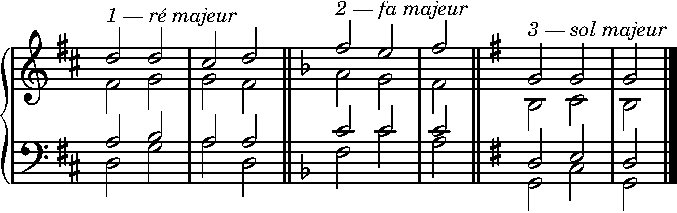
\includegraphics[scale=\echelle]{ca-exercice-1.cropped.pdf}\\[10pt]
  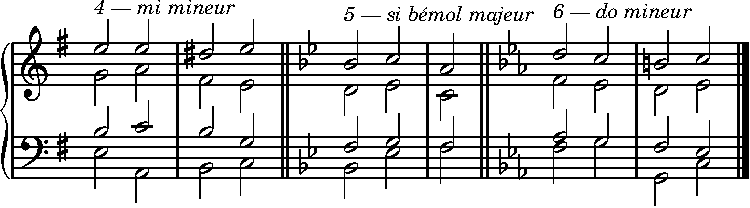
\includegraphics[scale=\echelle]{ca-exercice-2.cropped.pdf}
\end{minipage}\par\medskip

\par\medskip\noindent
\begin{minipage}{\linewidth}
  \textbf{Réaliser.} Écrire les voix du dessus sur ces basses chiffrées : 1, en
  sol majeur, en style clavier, trois sons à la main droite en position de
  tierce ; 2, en ré mineur, et 3, en fa majeur, à quatre voix, deux par main.

  \medskip
  \centering
  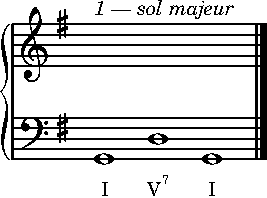
\includegraphics[scale=\echelle]{ca-exercice-realiser-1.cropped.pdf}\\[10pt]
  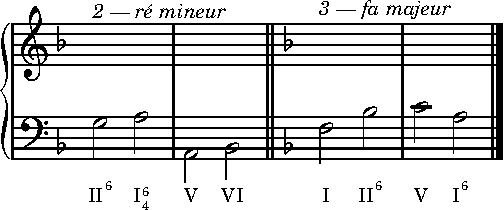
\includegraphics[scale=\echelle]{ca-exercice-realiser-2.cropped.pdf}
\end{minipage}\par\medskip

\textbf{Écouter.} Les six dernières entrées du fichier MusicXML, \emph{Écoute 1}
à \emph{Écoute 6}, font entendre six enchaînements courants, dans des
tonalités variées et sans leur nom. Retrouver les chiffres de chacun, puis
nommer la cadence qui le termine.

% Les réponses peuvent se couper d'une page à l'autre, plutôt que de laisser
% une demi-page vide.
\begin{remarque}[nobreak=false]
%% Produit par outils/generer_cadences.py — ne pas modifier à la main.
\textbf{Reconnaître.}
\begin{enumerate}[leftmargin=*, itemsep=1pt]
  \item \ch{I}{}{}--\ch{IV}{}{}--\ch{V}{7}{}--\ch{I}{}{}~: cadence parfaite.
  \item \ch{I}{}{}--\ch{V}{}{}--\ch{I}{6}{}~: cadence imparfaite.
  \item \ch{I}{}{}--\ch{IV}{}{}--\ch{I}{}{}~: cadence plagale.
  \item \ch{I}{}{}--\ch{IV}{}{}--\ch{V}{}{}--\ch{VI}{}{}~: cadence rompue.
  \item \ch{I}{}{}--\ch{II}{6}{}--\ch{V}{}{}~: demi-cadence.
  \item \ch{II}{6}{}--\ch{I}{6}{4}--\ch{V}{7}{}--\ch{I}{}{}~: cadence parfaite.
\end{enumerate}
\textbf{Écouter.} 1~: \ch{II}{6}{}--\ch{I}{6}{4}--\ch{V}{7}{}--\ch{I}{}{}, en sol majeur (cadence parfaite)~; 2~: \ch{I}{}{}--\ch{IV}{}{}--\ch{V}{}{}--\ch{VI}{}{}, en ré mineur (cadence rompue)~; 3~: \ch{I}{}{}--\ch{II}{6}{}--\ch{V}{}{}--\ch{I}{6}{}, en fa majeur (cadence imparfaite)~; 4~: \ch{I}{}{}--\ch{IV}{}{}--\ch{II}{6}{}--\ch{V}{}{}, en mi mineur (demi-cadence)~; 5~: \ch{I}{}{}--\ch{IV}{}{}--\ch{I}{}{}, en si bémol majeur (cadence plagale)~; 6~: \ch{I}{}{}--\ch{IV}{}{}--\ch{V}{7}{}--\ch{I}{}{}, en la mineur (cadence parfaite).


\textbf{Réaliser.} La première basse en style clavier, les deux autres à
quatre voix, deux par main :

\smallskip
\centering
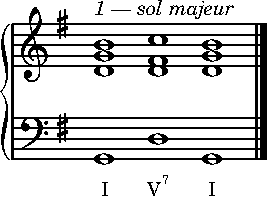
\includegraphics[scale=\echelle]{ca-reponse-realiser-1.cropped.pdf}\\[8pt]
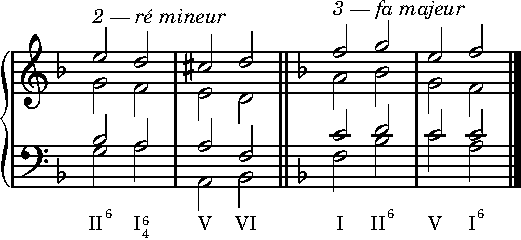
\includegraphics[scale=\echelle]{ca-reponse-realiser-2.cropped.pdf}
\end{remarque}

% =====================================================================
\section{Le fichier MusicXML}
\label{sec:musicxml}

Le fichier joint, \texttt{cadences.musicxml}, garde les deux dispositions, sur
une grande portée de piano, un accord par blanche à la noire 80 : les exemples
à quatre voix, deux par main ; puis les exemples du style clavier,
I--\ch{V}{7}{}--I en do majeur, en la majeur et en la mineur et I--IV--V--I
dans les trois positions ; enfin les six enchaînements de l'exercice
d'écoute. Il se lit avec MuseScore, Finale, Sibelius, Dorico ou tout éditeur
de partitions ; sur slashbin.net, il s'écoute aussi dans Sodor Piano. Chaque
main y joue ses voix en accords, et l'unisson du ténor et de la basse y sonne
une fois. Les chiffres n'y figurent pas : il sert à entendre ce qu'une cadence
suspend ou conclut.

Un second fichier, \texttt{cadences-tonalites.musicxml}, fait entendre
I--IV--V--I et I--\ch{V}{7}{}--I en style clavier, en position d'octave, dans
les trente tonalités des tableaux : chaque majeur, puis son homonyme mineur.
Les trois positions l'auraient triplé sans rien apprendre de plus à
l'oreille ; elles restent dans les tableaux.

% =====================================================================
\section*{Colophon}
\addcontentsline{toc}{section}{Colophon}

Les gravures musicales sont produites par \textbf{LilyPond}, la composition
par \textbf{\LaTeX}. Les enchaînements, les réponses des exercices et le
fichier MusicXML dérivent du modèle de hauteurs des autres guides, les modules
\texttt{gammes.py} et \texttt{intervalles.py} du dossier \texttt{outils}, et
de l'analyse des accords de \emph{Les accords}. Chaque enchaînement y est
réalisé dans l'une des deux dispositions de la section~\ref{sec:clavier} :
parmi les réalisations sans faute, celle où les voix parcourent le moins de
chemin. Il est ensuite relu à partir de ses seules notes : ses chiffres, ses
fautes éventuelles, le nom de sa cadence. Avant d'écrire quoi que ce soit, le
générateur vérifie dans les quinze tonalités majeures et les quinze mineures
ce que le texte affirme --- la sensible qui monte, la septième qui descend, la
quarte et sixte qui se résout, la tierce de VI doublée, aucune quinte ni
octave parallèle, chaque cadence reconnue sous son nom, la même disposition
dans toutes les tonalités d'un même mode ; en style clavier, la note commune
gardée, la main droite à l'opposé de la basse de IV à V, la quinte omise dans
\ch{V}{7}{} et le retour à la position de départ --- ; il vérifie aussi que
chaque exemple du style clavier donne exactement les accords gravés. Les deux
tableaux sortent des mêmes réalisations : chaque tonalité usuelle y a sa case,
une seule fois, chaque case est sans faute dans les trois positions, et les
cases vides sont exactement les six tonalités à plus de sept altérations. Pour
régénérer l'ensemble :

\begin{center}
\texttt{python3 outils/generer\_cadences.py}\\
\texttt{(cd gravures \&\& lilypond -dcrop --formats=pdf ca-*.ly)}\\
\texttt{pdflatex cadences.tex}
\end{center}

\end{document}
